\section{melcomp\_2}

Following VSS a slight alteration in approach occurred. Consideration was given to the $i_{\text{MB}}$ signal as a third dimension upon the already two-dimensional \gls{MB} chromaticity space, such as shown in figure \ref{fig:ZL}. This allowed the consideration what properties a signal upon this third dimension would need to provide to the overall three-dimensional point cloud in order for a transformation to occur which would transform the values into a two-dimensional illuminant-independent space.

\begin{figure}[htbp]
 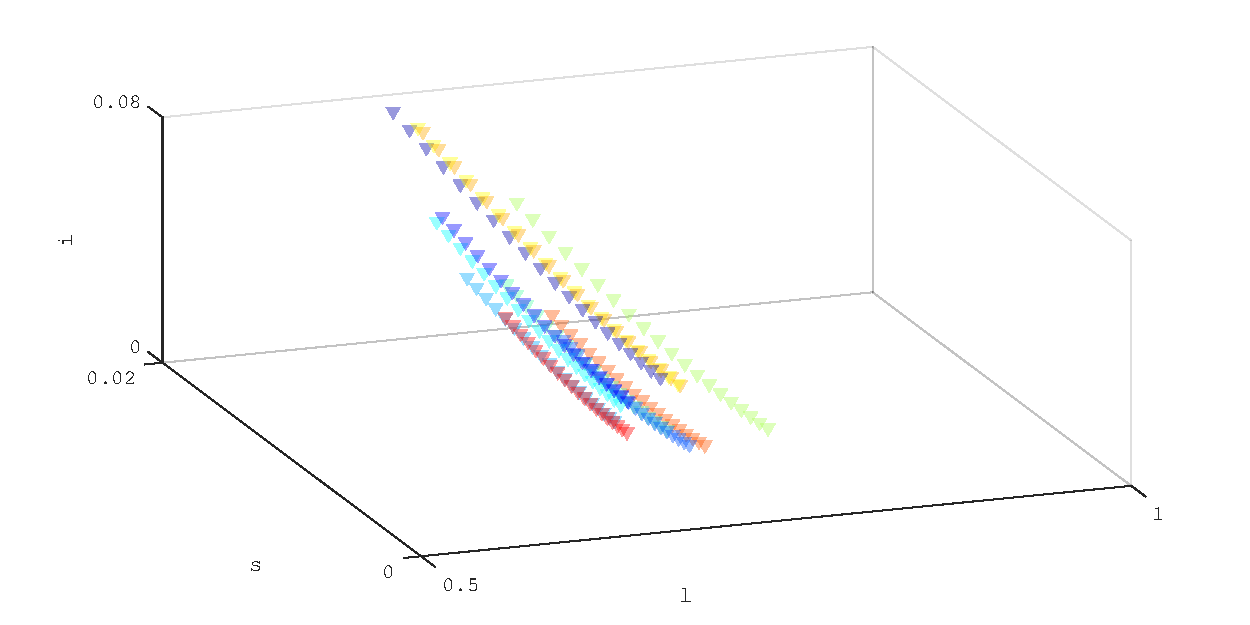
\includegraphics[max width=\textwidth]{figs/comp/melcomp_2/ZL.pdf}
 \caption{X and Y axes are a \gls{MB} chromaticity space, derived in this case using the \gls{SP} fundamentals, and the Z axis is $i_{\text{MB}}$. Plotted are the values for 11 surfaces (as per melcomp\_1), under 20 D-series illuminants (non-linear range between 3600 and 25000).}
 \label{fig:ZL}
\end{figure} % Update axes to add `MB'

The script started with the same process as melcomp\_1, loading data and computing \gls{MB} chromaticities, along with hypothetical $i_{\text{MB}}$ values. $r_{\text{MB}}$ values, the rod based analogue, were also calculated, although this was done for completeness (again, following the influence of \cite{barrionuevo_contributions_2014}) rather than following a genuine belief that they could be involved.

In addition to the data considered in melcomp\_1, support was added to inlcude a range of CIE D series illuminants\footnote{Generated with the \gls{PTB} function `GenerateCIEDay'.}, scenes 1-4 of the
\citet{nascimento_statistics_2002}\footnote{Data: \url{https://personalpages.manchester.ac.uk/staff/d.h.foster/Hyperspectral_images_of_natural_scenes_02.html}} hyperspectral reflectance data,
scenes 1-5 of the 
\citet{foster_frequency_2006}\footnote{Data: \url{https://personalpages.manchester.ac.uk/staff/d.h.foster/Hyperspectral_images_of_natural_scenes_04.html}}
hyperspectral reflectance data, and the \gls{SP} fundamentals\footnote{Loaded through \gls{PTB} as `T\_cones\_sp' (the new version as of \url{https://github.com/Psychtoolbox-3/Psychtoolbox-3/commit/2d360a2e827ed03174206cada5717ee555c727a1}).}. The CIE D-series illuminants allowed for a smaller and more controlled dataset, the Foster et al. data allowed for a more realistic distribution of reflectances and the \acrfull{SP} fundamentals allowed for a technically `correct' \gls{MB} diagram (before I knew about CIE 170-2:2015 \cite{cie_cie_2015}).

It was found that a log transform applied to the $[lsi]_{\text{MB}}$ data made relationships between the various signals more linear.

The key finding at this stage was that there is a perspective upon a three-dimensional point cloud ($[l_{\text{MB}},s_{\text{MB}},i_{\text{MB}}]$) from which points from like objects clustered well, such as in figure \ref{fig:viewpoint}. This property shows that there is at least one transformation such that the points could be projected upon a two-dimensional plane where the illuminant-dependence was greatly reduced whilst the inter-object chromatic relationships were retained. 

\begin{figure}[htbp] % redo this. Is this log data?
 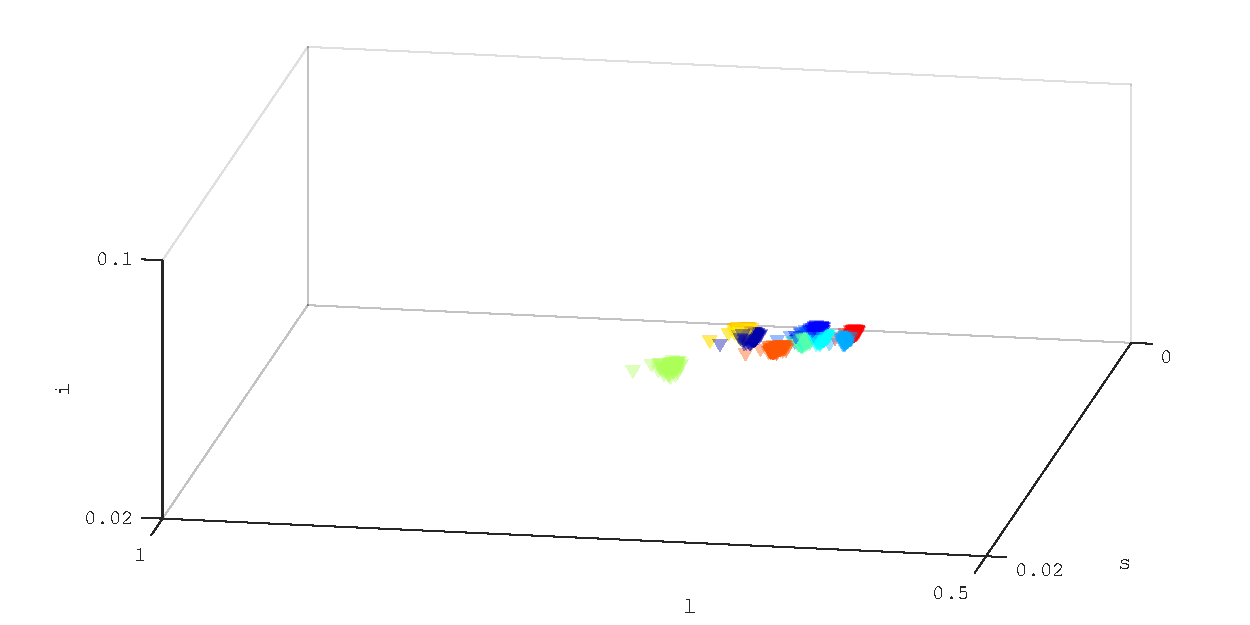
\includegraphics[max width=\textwidth]{figs/comp/melcomp_2_caller/viewpoint.pdf}
 \caption{Figure \ref{fig:ZL} rotated to a perspective where it can be seen that the points project upon a two-dimensional plane in a clustered fashion whilst not degrading to a line within that space.}
 \label{fig:viewpoint}
\end{figure} 

Note that such a perspective would not be possible for a space where the third dimension were a near-duplicate of the first or second, since in this case all points would lie upon a plane. This would be the case in circumstances where a corrective signal too closely resembled the visual signals, as we found at the end of melcomp\_1. The fact that points do not lie on a plane shows that there is some decorrelation between $i_{\text{MB}}$ and both $l_{\text{MB}}$ and $s_{\text{MB}}$. The fact that they do not lie on a plane and instead diverge from this plane in a surface-dependent fashion (as opposed to noisily diverging) suggests that the $i_{\text{MB}}$ may present a means to separate the contribution from illuminant and surface. 

Following this, a range of speculative transformations were performed, to demonstrate the types of transformation that could be used to transform colour signals to illuminant-independent colour signals. A rotational transformation was successful (analogous to changing the perspective as in figure \ref{fig:viewpoint}) and additionally a weighted additive model was found to be more-or-less successful. No satisfactory model was found where a purely multiplicative transformation was applied.

Thinking about a corrective signal as an additional dimension upon a \gls{MB} chromaticity space allows for consideration of requisite or desirable properties that this third signal should imbue upon the three-dimensional cloud of points. I have identified one requisite property, and one desirable property. 

The requisite property for such a signal, as already suggested, is that it should differ from other chromatic signals enough to allow for the point cloud of chromatic points to be significantly \emph{non-planar}. This in turn allows for a projection upon two-dimensional space which has the potential to be illuminant-invariant.

The desirable property is that it should be \emph{roughly monotonic} with respect to other chromatic signals. This allows a one-to-one mapping of colour signals to illuminant-independent colour signals, where a non-monotonic relationship does not necessarily do so. This is not a strict requirement, since the corrective function only needs to be one directional, but non-monotonicity would exclude simple transforms (such as linear additive or rotational).

At this stage the underlying reason for the relative success of these transforms was considered. One potential lead is a curious regularity at the lower wavelengths of the reflectance spectrum of many natural objects. In figure \ref{fig:plateau} it can be seen that there is a plateau in the relative spectral reflectances of some natural objects (a subset of the \citet{vrhel_measurement_1994} reflectances) between roughly 430nm and 480nm, with relatively small deviations within 400nm to 500nm. Another way to visualise this is to calculate the correlation between points on the reflectance function. Such a calculation was performed initially on a combined set of scenes 1-4 of the
\citet{nascimento_statistics_2002}\footnote{Data: \url{https://personalpages.manchester.ac.uk/staff/d.h.foster/Hyperspectral_images_of_natural_scenes_02.html}} hyperspectral reflectance data and
scenes 1-5 of the 
\citet{foster_frequency_2006}\footnote{Data: \url{https://personalpages.manchester.ac.uk/staff/d.h.foster/Hyperspectral_images_of_natural_scenes_04.html}}
hyperspectral reflectance data, and then on three other datasets. See figure \ref{fig:foster} and \ref{fig:others} respectively.

\begin{figure}[htbp]
 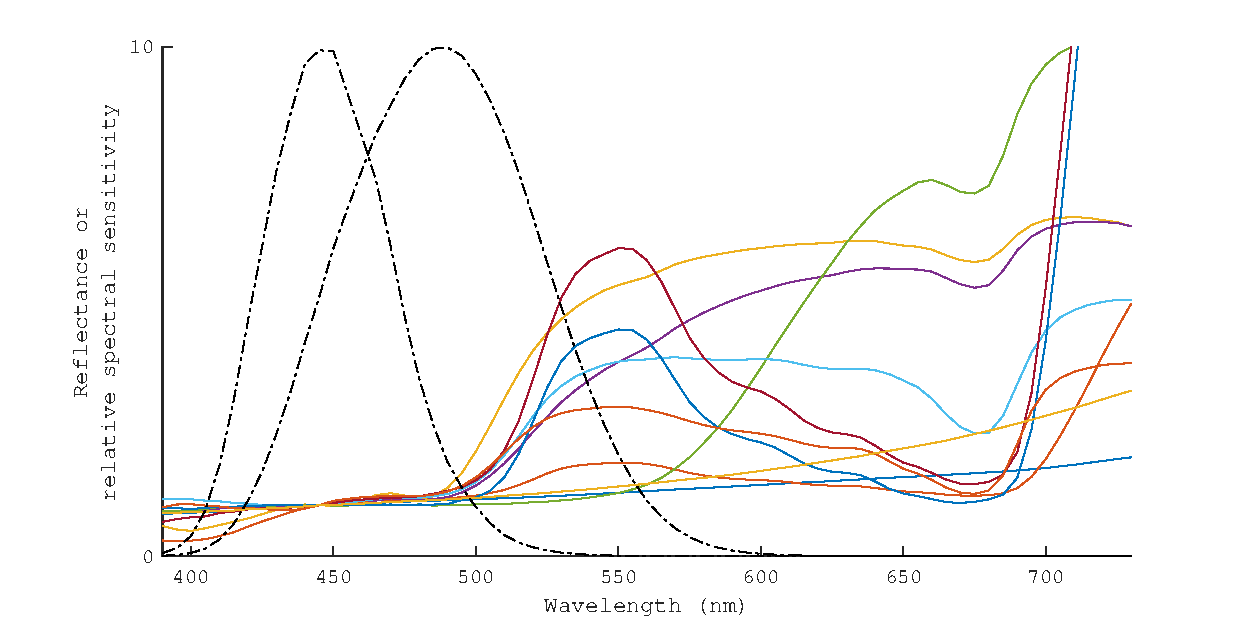
\includegraphics[max width=\textwidth]{figs/comp/melcomp_2_caller/plateau.pdf}
 \caption{The spectral reflectance functions of a subset of the \citet{vrhel_measurement_1994} reflectances (solid lines), normalised at the peak of s-cone sensitivity (CIE 2006 10$^{\circ}$), with the spectral sensitivity of s-cones and melanopsin \citep{lucas_measuring_2014} overlaid (dot-dashed lines).}
 \label{fig:plateau}
\end{figure} 

\begin{figure}[htbp]
 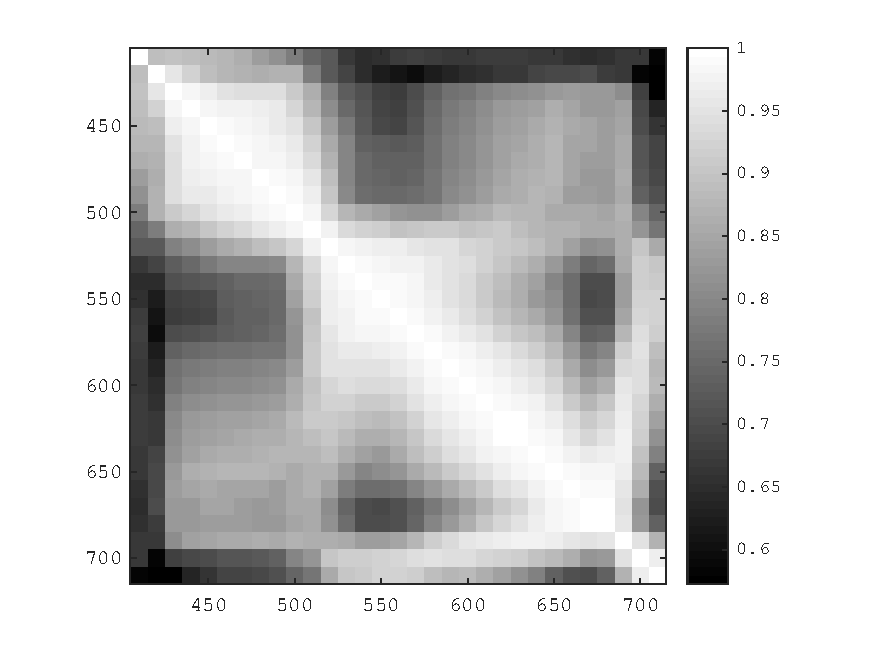
\includegraphics[max width=\textwidth]{figs/comp/nat_cor/foster.pdf}
 \caption{Visualisation of the average correlation matrix for the scenes 1-4 of \citep{nascimento_statistics_2002} and 1-5 of \citep{foster_frequency_2006}. Note the rough square in the top left, indicating an area of increased correlation across different wavelength samplings, and another rough square (though with a faded lower-right corner) in the centre. The dark frame to this figure is likely due to increased measurement noise at these extremes.}
 \label{fig:foster}
\end{figure} %get rid of dotted line on colorbar

\begin{figure}[htbp]
 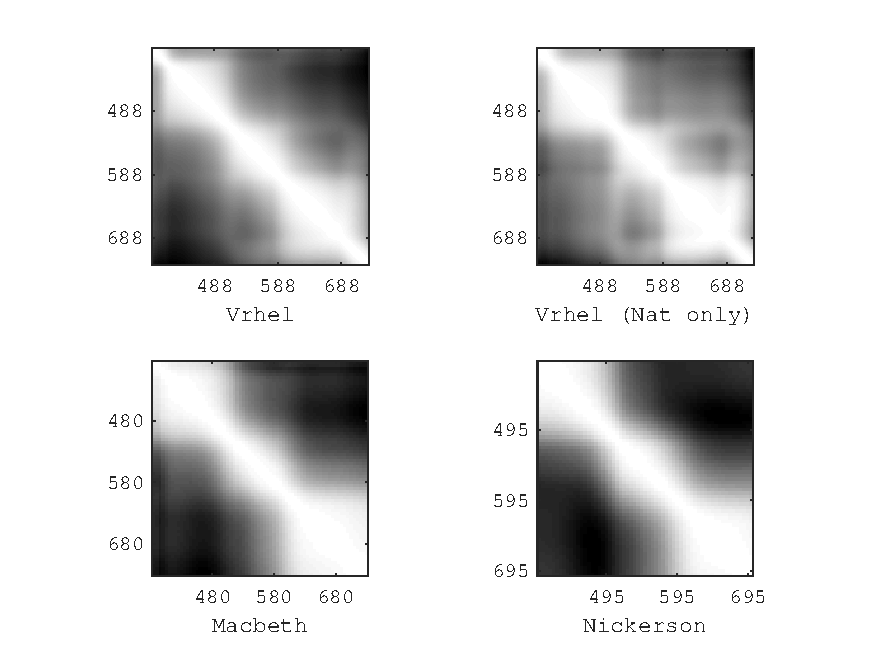
\includegraphics[max width=\textwidth]{figs/comp/nat_cor/others.pdf}
 \caption{As for \ref{fig:foster} but for 3 different sets of data, and one subset. `Vrhel' refers to the object reflectances of \citet{vrhel_measurement_1994} data and `Vrhel (nat only)' refers to a subset of the previous but only using data for surfaces which were deemed `natural'. `Macbeth' refers to measurements of a Macbeth Color Checker. `Nickerson' refers to a set of measurements of Munsell papers (presumably the \citet{kelly_tristimulus_1943} data). Note that whilst we have a selection of real surfaces, natural surfaces, and printed papers, all plots show similar trends, with three areas of correlation, at low, medium and high wavelengths. The low wavelength square seems to match that in Figure \ref{fig:foster} well, but the other two areas are only really distinguishable in this second set of figures. All data obtained via \gls{PTB} (`sur\_vrhel', `sur\_macbeth', `sur\_nickerson').}
 \label{fig:others}
\end{figure} 

An interesting advantage could be made of this regularity. Assume a simpler situation where there were two points on the spectrum of the reflectance functions of a set of natural objects which were always the same as eachother (perfect correlation). Sensors of appropriately narrow spectral sensitivity, placed at these two points on the spectrum would always register corresponding signals. Considering that the second principal component of daylight variability is a broad skew, any difference in the signals from two such receptors could be used fairly reliably to sense the contribution of this second component in any single condition. 

This work was presented at this stage as a poster at the \emph{Visual Neuroscience Summer School (Rauischholzhausen, 2018)} as a poster, which has not been made publicly available.

To summarise melcomp\_2:

\begin{enumerate}
    \item A perspective upon the three-dimensional $[lsi]_{\text{MB}}$ space was found where points diverged from a plane in a surface-dependent fashion. \emph{Figure \ref{fig:viewpoint}}
    \item One requisite and one desirable property for a hypothetical third signal were identified: decorrelation (leading to non-planarity) and monotonicity. 
    \item The underlying reason for the relative success of the investigated transforms was considered. A plateau at shorter wavelengths of natural object reflectances was noted, and it was speculated that this could be taken advantage of.
\end{enumerate}
